%==============================================================================
% Chapitre 26 - Centre de gravité
%==============================================================================

\section{Introduction}

Lorsqu'on observe un projectile, il est naturel de considérer sa masse comme
uniformément répartie.

Dans la réalité, la matière est distribuée dans un volume donné et cette
répartition influence directement le comportement du projectile.

Afin de simplifier l'étude mécanique des corps, on introduit la notion de
centre de gravité.

Cette notion joue un rôle essentiel en balistique.

\begin{aretenir}

Le centre de gravité représente le point d'application résultant du poids
d'un corps.

\end{aretenir}

\section{Définition}

Le centre de gravité est le point où l'on peut considérer que l'ensemble du
poids du projectile est appliqué.

Dans un champ de gravité uniforme, il coïncide avec le centre de masse.

Pour les dimensions considérées en balistique, cette approximation est
parfaitement valable.

Dans la suite du document, les termes centre de gravité et centre de masse
seront souvent utilisés de manière interchangeable.

\begin{figure}[htbp]
\centering
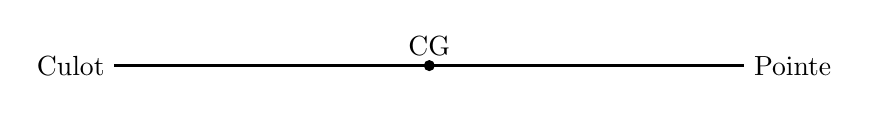
\begin{tikzpicture}

\draw[thick] (0,0) -- (8,0);

\fill (4,0) circle (2pt);

\node[above] at (4,0) {CG};

\node[left] at (0,0) {Culot};
\node[right] at (8,0) {Pointe};

\end{tikzpicture}
\caption{Position du centre de gravité d'un projectile.}
\label{fig:centre_gravite}
\end{figure}


\section{Exemple intuitif}

Prenons une règle.

Si l'on cherche à l'équilibrer sur un doigt, il existe une position
particulière où elle reste horizontale.

Cette position correspond au centre de gravité.

La même idée s'applique aux projectiles.

\section{Répartition de la masse}

Le centre de gravité dépend directement de la manière dont la masse est
répartie.

Deux projectiles de même forme extérieure peuvent posséder des centres de
gravité différents si leur structure interne diffère.

Par exemple :

\begin{itemize}
    \item noyau en plomb ;
    \item noyau en acier ;
    \item noyau en tungstène ;
    \item cavité interne.
\end{itemize}

\section{Projectile homogène}

Dans un projectile constitué d'un matériau uniforme et de forme symétrique,
le centre de gravité est généralement situé sur l'axe de symétrie.

Pour un cylindre homogène :

\begin{itemize}
    \item il se situe au milieu de la longueur.
\end{itemize}

\section{Projectile réel}

Les projectiles modernes sont rarement homogènes.

Ils comportent souvent :

\begin{itemize}
    \item plusieurs matériaux ;
    \item une chemise ;
    \item un noyau ;
    \item des cavités ;
    \item des éléments pyrotechniques.
\end{itemize}

Le centre de gravité doit alors être déterminé par calcul ou mesure.

\section{Position du centre de gravité}

La position du centre de gravité est généralement exprimée par rapport :

\begin{itemize}
    \item à la pointe ;
    \item au culot ;
    \item à la longueur totale du projectile.
\end{itemize}

Cette position constitue un paramètre important pour les études de stabilité.

\section{Calcul du centre de gravité}

Pour un système composé de plusieurs masses :

\begin{equation}
x_G =
\frac{\sum m_i x_i}
     {\sum m_i}
\end{equation}

où :

\begin{itemize}
    \item $x_G$ est la position du centre de gravité ;
    \item $m_i$ représente une masse ;
    \item $x_i$ représente sa position.
\end{itemize}

\section{Exemple simplifié}

Considérons un projectile constitué de deux masses :

\begin{itemize}
    \item 6 g situés à 10 mm ;
    \item 4 g situés à 20 mm.
\end{itemize}

Le centre de gravité est :

\begin{equation}
x_G =
\frac{(6 \times 10)+(4 \times 20)}
     {6+4}
=
14~mm
\end{equation}

Il est donc situé plus près de la masse la plus importante.

\section{Mesure expérimentale}

Le centre de gravité peut être mesuré expérimentalement.

Les méthodes les plus courantes consistent à :

\begin{itemize}
    \item équilibrer le projectile ;
    \item utiliser des dispositifs de suspension ;
    \item effectuer des mesures géométriques.
\end{itemize}

\section{Influence sur le vol}

La position du centre de gravité influence fortement :

\begin{itemize}
    \item la stabilité ;
    \item les moments aérodynamiques ;
    \item la réponse aux perturbations.
\end{itemize}

Cependant, le centre de gravité seul ne suffit pas à prédire le comportement
du projectile.

Il doit être étudié conjointement avec le centre de pression.

\section{Pourquoi avancer le centre de gravité ?}

Dans de nombreux projectiles modernes, les concepteurs cherchent à placer le
centre de gravité relativement vers l'avant.

Cette disposition tend généralement à améliorer certaines caractéristiques
de stabilité.

Les raisons exactes apparaîtront dans les chapitres suivants.

\section{Centre de gravité et rotation}

La rotation du projectile s'effectue autour de son axe longitudinal.

La position du centre de gravité influence :

\begin{itemize}
    \item les moments d'inertie ;
    \item la stabilité gyroscopique ;
    \item la précession.
\end{itemize}

Nous reviendrons sur ces notions ultérieurement.

\section{Centre de gravité et simulation}

Les modèles balistiques simples ignorent souvent la position exacte du centre
de gravité.

Les modèles avancés l'utilisent explicitement.

Cette information devient indispensable dans les modèles :

\begin{itemize}
    \item 4DOF ;
    \item 5DOF ;
    \item 6DOF.
\end{itemize}

\begin{simulation}

Dans un modèle de masse ponctuelle, le centre de gravité est confondu avec
le projectile lui-même.

Dans un modèle 6DOF, sa position influence directement les équations du
mouvement.

\end{simulation}

\section{Vers le centre de pression}

Connaître le centre de gravité ne suffit pas.

Pour comprendre pourquoi un projectile est stable ou instable, il faut
également connaître le point d'application des forces aérodynamiques.

Ce point est appelé centre de pression.

Sa position relative par rapport au centre de gravité constitue l'une des
clés de la stabilité en vol.

\section{À retenir}

\begin{aretenir}

\begin{itemize}
    \item Le centre de gravité dépend de la répartition des masses.
    \item Il coïncide généralement avec le centre de masse.
    \item Sa position influence fortement la stabilité.
    \item Les projectiles modernes ne sont pas homogènes.
    \item Le centre de gravité doit être étudié conjointement avec le centre
    de pression.
\end{itemize}

\end{aretenir}
